%%%%%%%%%%%%%%%%%%%%%%%%%%%%%%%%%%%%%%%%%
% Diaz Essay
% LaTeX Template
% Version 2.0 (13/1/19)
%
% This template originates from:
% http://www.LaTeXTemplates.com
%
% Authors:
% Vel (vel@LaTeXTemplates.com)
% Nicolas Diaz (nsdiaz@uc.cl)
%
% License:
% CC BY-NC-SA 3.0 (http://creativecommons.org/licenses/by-nc-sa/3.0/)
%
%%%%%%%%%%%%%%%%%%%%%%%%%%%%%%%%%%%%%%%%%

%----------------------------------------------------------------------------------------
%	PACKAGES AND OTHER DOCUMENT CONFIGURATIONS
%----------------------------------------------------------------------------------------

\documentclass[11pt]{diazessay} % Font size (can be 10pt, 11pt or 12pt)
\usepackage{amsmath,amssymb}
\DeclareMathOperator{\E}{\mathbb{E}}
\usepackage{graphicx}
\graphicspath{ {../} }

%----------------------------------------------------------------------------------------
%	TITLE SECTION
%----------------------------------------------------------------------------------------

\title{\textbf{Final Project of Numerical Methods for PDE} \\ {\Large\itshape Finite Volume Method for Euler Equation}} % Title and subtitle

\author{\textbf{Zejian You} \\ \textit{Columbia University}} % Author and institution

\date{\today} % Date, use \date{} for no date

%----------------------------------------------------------------------------------------

\begin{document}

\maketitle % Print the title section

%----------------------------------------------------------------------------------------
%	ABSTRACT AND KEYWORDS
%----------------------------------------------------------------------------------------

%\renewcommand{\abstractname}{Summary} % Uncomment to change the name of the abstract to something else
%----------------------------------------------------------------------------------------
%	ESSAY BODY
%----------------------------------------------------------------------------------------
\section{Problem Description}

- Mass Conservation
  
$$\rho_t + (\rho u)_x = 0.$$

- Momentum Conservation

$$(\rho u)_t + (\rho u^2 + p)_x = 0.$$

- Energy Conservation
  
$$E = \rho e + \frac{1}{2}\rho u^2.$$
$$E_t + (u(E+p))_x = 0.$$

To close the equation system, we need one more equation

- Equation of State
$$
p = \rho e(\gamma -1)
$$

\subsection{Hyperbolic structure of the 1D Euler equations}
The governing equation could be written into a system of hyperbolic equations:
$$
    \frac{\partial \bf{q}}{\partial t} + \frac{\partial \bf{F}(\bf{q})}{\partial x} =0 \quad \text{or}
$$
$$
    \bf{q} = \begin{bmatrix}
        \rho \\ \rho u\\ E
    \end{bmatrix}, \quad \bf{F}(\bf{q})=\begin{bmatrix}
        \rho u \\\rho u^2 + p\\(E + p) u
    \end{bmatrix}
$$

\subsection{Finite Volume Method}
Based on Green's formula, we have

$$
\nabla\cdot \textbf{F}(\textbf{V}) = \oint_{\partial T_j} \textbf{F}(\textbf{V})\cdot \textbf{n} ds
$$

For finite volume discretization, we have\cite{li_multigrid_nodate}

$$
\oint_{\partial T_j} \textbf{F}(\textbf{V})\cdot \textbf{n} ds 
\approx \sum_{e_{ik}\in \partial T_j} \oint_{e_{jk}} \bar{\textbf{F}}(\textbf{V}_j, \textbf{V}_k)\cdot \textbf{n}_{jk} dl
$$


\begin{align}
    Q_j^{n+1} = Q_j^n - \frac{\Delta t_n}{\Delta x_j} (F_{j+1/2}^n - F_{j-1/2}^n)
\end{align}

\subsection{Eigenvalue and Eigenvector of Euler Flux Jacobian}

    Flux of variable $\textbf{q}$ equal to
    
    $$
    \begin{aligned}
        \bar{\textbf{F}}(\textbf{q})= \begin{bmatrix}
            q_2\\ 
            \frac{q_2^2}{q_1} + \left(q_3 - \frac{q_2^2}{2q_1}\right) (\gamma -1)\\
            \frac{\gamma q_2q_3}{q_1} - \frac{q_2^3}{2q_1^2}(\gamma -1)
        \end{bmatrix}
    \end{aligned}
    $$


    Flux Jacobian of variable $\textbf{V}$ equal to \footnote{with $p = (E - \frac{1}{2}\rho u^2)(\gamma -1)$, and $H=\frac{E+p}{\rho}$}

    $$
    \begin{aligned}
        \frac{\partial \bar{\textbf{F}}(\textbf{q})}{\partial \textbf{q}}= \begin{bmatrix}
            u & 1 & 0 \\
            \frac{\gamma -3}{2} u^2 & (3-\gamma)u & \gamma -1\\
            \frac{\gamma -1}{2}u^3-uH & H-(\gamma -1)u^2 & \gamma u\\
        \end{bmatrix}
    \end{aligned}
    $$

    Then the Euler Equation becomes 

    $$
    \textbf{q}_t + \frac{\partial \bar{\textbf{F}}(\textbf{q})}{\partial \textbf{q}}\textbf{q}_x= 0
    $$

    The eigenvalues and corresponding eigenvectors of Jacobian matrix is
    $$
    \begin{aligned}
        & \lambda_1 = u -c, &&\lambda_2 = u,\quad && \lambda_3 = u+c\\
        &\textbf{r}_1 =\begin{bmatrix} 1 \\ u-c \\H-uc\end{bmatrix}
        &&\textbf{r}_2 =\begin{bmatrix} 1 \\ u \\ \frac{1}{2}u^2 \end{bmatrix}\quad
        &&\textbf{r}_3 =\begin{bmatrix} 1\\ u+c \\H+uc\end{bmatrix}
    \end{aligned}
    $$

    Here $c=\sqrt{(\gamma - 1)(H-\frac{1}{2}u^2)}$.    \cite{david_i_ketcheson_chapter_2020, roe_approximate_1981}

\section{Riemann Problem}
\subsection{Linearized Riemann Solver}

Besides the exact Riemann solution, we could also obtain an approximate solution by linearizing the Euler Equation and replacing Jacobian of flux $\frac{\partial \bf{F}(\textbf{q})}{\partial \bf{q}}$ by a linear operator $\hat{\bf{A}}(q_l, q_r)$ depending on the left and right status \cite{roe_approximate_1981}. Furthermore, this approximate linear operator should satisfy:


\begin{enumerate}

\item Consistency: $\hat{\bf{A}}(\textbf{q}_l, \textbf{q}_r) \rightarrow \textbf{F}'(\textbf{q})$ as $\textbf{q}_l, \textbf{q}_r \rightarrow \textbf{q}$
\item Hyperbolicity: $\hat{\bf{A}}$ must be diagonalizable with real eigenvalues, so that we can define the waves and speeds needed in the approximate solution.
\item Conservation: 
\begin{equation}\label{eq:conservation}
\hat{\bf{A}}(\textbf{q}_l, \textbf{q}_r)(\textbf{q}_r-\textbf{q}_l) = \textbf{F}(\textbf{q}_r) - \textbf{F}(\textbf{q}_l)
\end{equation}
\end{enumerate}


One common linear operator is the flux Jacobian of an average state:

\begin{equation}\label{eq:linearization}
    \hat{\bf{A}}(\textbf{q}_l, \textbf{q}_r) = \textbf{F}'(\hat{\textbf{q}})\text{, }\quad \hat{\textbf{q}}\in[\textbf{q}_l, \textbf{q}_r]
\end{equation}

Plugged Eq.(\ref{eq:linearization}) back into Eq.(\ref{eq:conservation}), we have


\begin{equation}\label{eq:AverageState}
    \textbf{F}'(\hat{\textbf{q}})(\textbf{q}_r-\textbf{q}_l) = \textbf{F}(\textbf{q}_r) - \textbf{F}(\textbf{q}_l)
\end{equation}

Solve Eq.(\ref{eq:AverageState}), we could obtain the Roe average state expression

\begin{equation}
    \bar{u} = \frac{\sqrt{\rho_r}u_r + \sqrt{\rho_l}u_l}{\sqrt{\rho_r}+\sqrt{\rho_l}}, \quad \bar{H} =\frac{\sqrt{\rho_r}H_r + \sqrt{\rho_l}H_l}{\sqrt{\rho_r}+\sqrt{\rho_l}}
\end{equation}

For the system of hyperbolic equations, we could solve the system by decomposing the linear operator $\hat{\bf{A}}$ into the eigenvectors $\bf{R}$ and the matrix that eigenvalues on the diagonal $\bf{\Lambda}$ so that

$$
\begin{aligned}
    \bf{q}_t + \hat{\bf{A}} \bf{q}_x  &= 0\\
    \bf{q}_t + \bf{R}\Lambda\bf{R}^{-1}\bf{q}_x & = 0\\
    \bf{R}^{-1}\bf{q}_t + \Lambda\bf{R}^{-1}\bf{q}_x & = 0\\
    \bf{w}_t + \Lambda\bf{w}_x & = 0\\
    w_k(x, t) & = w_k(x-\lambda_k t, 0)\\
    \bf{q}(x, t) & = \sum_k w_k(x-\lambda_k t, 0) \bf{r_k}
\end{aligned}
$$


\subsection{Two-wave solver}

Instead of linearization, we could also approximate the solution to be one wave propagating in each direction based on previous analysis of Euler Equations. Thus, there will be only one intermediate state $q_m$ in this situation, which satisfies $\mathcal{W}_1=\textbf{q}_m-\textbf{q}_l$ and $\mathcal{W}_2=\textbf{q}_r-\textbf{q}_m$. Thus,


\begin{equation}\label{eq:TwoWaveAverage}
    \textbf{F}(\textbf{q}_r) - \textbf{F}(\textbf{q}_l) = s_1\mathcal{W}_1 + s_2\mathcal{W}_2
\end{equation}


in which $s_1$ and $s_2$ are the corresponding wave speeds.

From Eq.(\ref{eq:TwoWaveAverage}), we could obtain the expression for the intermediate state

\begin{equation}
    \label{eq:TwoWaveIntermediate}
    q_m = \frac{\textbf{F}(\textbf{q}_r)-\textbf{F}(\textbf{q}_l) + s_1\textbf{q}_l - s_2\textbf{q}_r}{s_1 - s_2}
\end{equation}




\subsubsection{Lax-Friedrichs Numerical Flux}

The simpliest method is Lax-Friedrichs method. This method assumes that the wave speeds have the same value but different signs. $s_1 = -s_2 = a$. Furthermore, the wave speed is chosen by the maximum of flux for q over $\textbf{q}_l$ and $\textbf{q}_r$:

\begin{equation}
    a =  max(|\textbf{F}'(\textbf{q})|)
\end{equation}

\subsubsection{Harten-Lax-van Leer (HLL)}

This method assumes that wave speeds are different but still based on the maximum and minimum of the flux:

\begin{equation}
    s_1 =  \min(\textbf{F}'(\textbf{q})) \quad \mbox{and}\quad s_2 =  \max(\textbf{F}'(\textbf{q}))
\end{equation}


\section{Conclusion}

The numerical solver of Euler Equations by Roe flux, Lax-Friendrichs numerical Flux and HLL scheme can be coded up based on previous information and the exact solution is imported from previous work\cite{david_i_ketcheson_chapter_2020}. 

We could see that the approximate solution by roe flux is represented by three propagating wave while the solutions obtained by two waves solver have only two waves. Furthermore, the left going rarefaction wave is replaced by a shock wave in both solver. However, it should be noticed that the two waves solver adopted the maximum wave speed should have the same intermediate domain with exact solver while in my result, the right going wave is lagging behind the exact solution, which requires further investigation.

\begin{figure}[h!]
    \centering
    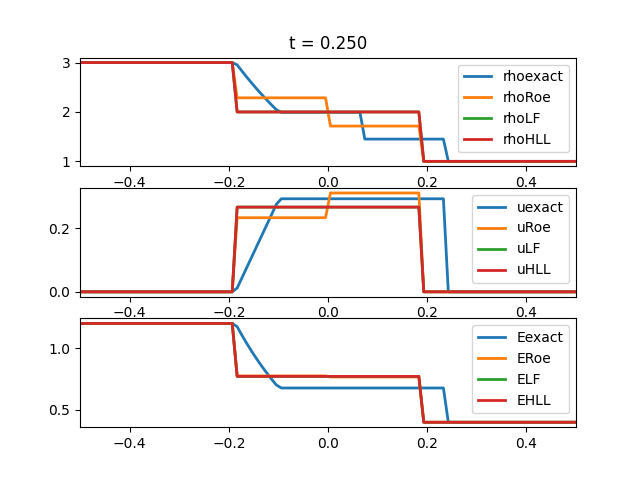
\includegraphics[scale=0.8]{comparison.png}
    \label{fig:shocktube}
    \caption{Comparison of Different Riemann Solver}
\end{figure}


\clearpage
%----------------------------------------------------------------------------------------
%	BIBLIOGRAPHY
%----------------------------------------------------------------------------------------
\bibliographystyle{unsrt}
\bibliography{../Euler.bib}

%----------------------------------------------------------------------------------------

\end{document}
